\documentclass[journal]{IEEEtran}
\usepackage[utf8]{inputenc}
\usepackage{graphicx}
\usepackage[hyphens]{url}

\title{An FPGA Implementation of a \\ Digital Storage Oscilloscope}
\author{Andrei~Purcarus~Craciun,~\IEEEmembership{McGill~University} and Ze~Yu~Yang,~\IEEEmembership{McGill~University}}

\begin{document}
\sloppy

\maketitle

\begin{abstract}

This paper discusses the design, implementation, testing and synthesis of a digital storage oscilloscope on the DE1-SoC Cyclone V FPGA development board. This oscilloscope is capable of capturing a waveform using an ADC, processing it in real-time and displaying it on a VGA monitor. It uses sin(x)/x interpolation to extend the range of frequencies for which waveforms can be properly displayed to 200~kHz for a 500~kSa/s ADC. It also uses an internal frequency counter to measure the trigger frequency of waveforms with at most 0.26~\% error over a range of frequencies from 1~kHz to 200~kHz. In addition, it provides measurements of the peak-peak, average, max and min voltages of captured waveforms with an error of at most 1~\%~+~10~mV using a 12-bit ADC whose range is 0.000~V to 4.095~V. Potential improvements and additions to the functionality of the oscilloscope are also discussed.

\end{abstract}

\begin{IEEEkeywords}

Digital storage oscilloscope, FPGA, real-time processing, sin(x)/x interpolation.

\end{IEEEkeywords}

\section{Introduction}

\IEEEPARstart{T}{he} purpose of this project is to implement the digital components of a digital storage oscilloscope (DSO) on an FPGA device. We will assume that the analog input circuitry is already available, with the processed analog signal having been converted to a digital signal through an ADC. We will target the Cyclone V DE1-SoC FPGA development board since this board contains the necessary hardware peripherals to implement an oscilloscope. Specifically, this board contains a 50~MHz base clock, a 12-bit, 500~kSa/s ADC and a 24-bit video DAC connected to a VGA D-Sub connector \cite{DE1SoC,ltc2308}. Therefore, our DSO can use the ADC to sample an input waveform and the video DAC to display the processed waveform on a VGA monitor.

This project is motivated by the fact that traditional DSOs use a microprocessor to perform their processing, and this tends to be a bottleneck for real-time processing and complex operations such as the FFT \cite{tektronix_xyz_2016}. We aim to eliminate this bottleneck by providing a pipelined, parallel implementation of the DSO functionality.

This functionality consists of capturing waveform data to an internal memory, and displaying the data when triggered by a predefined event. This event usually consists of the input waveform crossing a certain reference level with a positive or negative slope, referred to as rising edge and falling edge triggering, respectively \cite{tektronix_xyz_2016}. It is necessary to have this trigger for a stable waveform display, as it centers a periodic waveform on the same point over multiple video frames.

Although DSOs have been implemented on FPGAs before as student projects, the lack of proper interpolation led to a maximum displayable waveform frequency of 30~kHz using the same development board \cite{jin_digital_2016}. We aim to do better by using sin(x)/x interpolation techniques on the captured waveforms, which will theoretically allow us to perfectly reconstruct band-limited signals of frequencies less than 250~kHz, as given by the Nyquist criterion and our ADC sample rate. This is done by inserting zeros in between sample points (up-sampling), and applying a low-pass filter on the resulting waveform, which results in a perfect reconstruction of the waveform at the up-sampled points \cite{rehorn_sin_2009}.

For our design, we will aim for a maximum frequency of 200~kHz. This frequency was chosen to account for practical limitations in the interpolation algorithm. Since an ideal low-pass filter is impossible to achieve in practice, we will use a FIR filter with a finite roll-off. To avoid aliasing and ensure sufficient attenuation in the stop-band, we thus chose a lower cutoff frequency.

We will also aim for a minimum frequency of 1~kHz, which was chosen for simplicity as an order of magnitude higher than typical VGA frame rates of 60~Hz to 72~Hz \cite{vga_timing}. This will allow for multiple waveform captures over a single frame, and hence allow us to perform processing in real time.

In addition, although we will not be measuring the waveform frequency explicitly, we will measure the frequency at which the oscilloscope is triggered. This serves as a proxy for the waveform frequency, and will correctly identify it for waveforms with one trigger per period, such as sine and square waves. We will compare the accuracy of this measurement to the frequency measurement accuracy obtained by previous projects \cite{jin_digital_2016}. The resolution of our frequency measurement will be limited by the clock rate, and we will therefore aim for an accuracy of 1~\%~+~10~Hz over a frequency range of 1~kHz to 200~kHz.

Finally, we will perform voltage measurements on the captured waveform data, and output these to the display. We aim to produce peak-peak, average, max and min voltage measurements for the captured waveforms. Given that we have a 12-bit ADC with a range of 0.000~V to 4.095~V, we will aim for an accuracy of 1~\%~+~10 mV on these measurements over the entire frequency range. It is here that interpolation will really be tested since for higher frequencies the limited sampling rate means that we might not be able to capture the peaks of the waveform through the ADC. Hence we will rely on interpolation to produce these values, and compare them to the actual values.

For evaluation, the project will first be simulated using an analog waveform generator designed in a previous assignment for this course. The VGA output signals will be logged to a text file, and this text file will be used to view the VGA display using a simulator \cite{vga_sim}. Then, the project will be synthesized on the FPGA board and analog signals from a signal generator will be fed to the ADC and compared to the readouts on a commercial oscilloscope and multimeter.

\section{Design Methodology}

\begin{figure}[!htb]
  \centering
  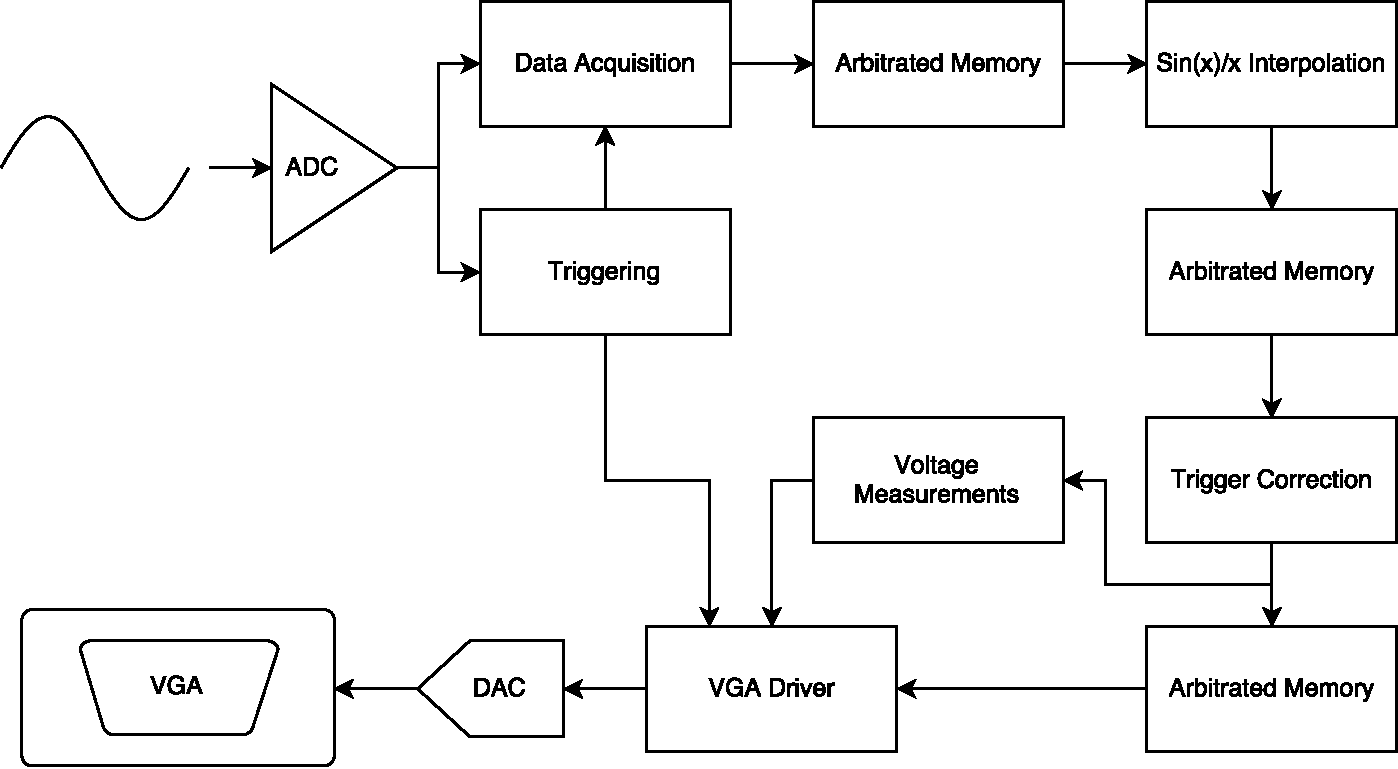
\includegraphics[width=\columnwidth]{diagrams/system.pdf}
  \caption{Simplified top-level block diagram of the DSO.}
  \label{fig:system}
\end{figure}

A simplified block diagram of the DSO is shown in Figure~\ref{fig:system}. The analog waveform we wish to capture is assumed to have been processed by external analog circuitry and sampled by an ADC.

This ADC signal is monitored by a triggering module which produces a trigger signal on a rising or falling edge of the input waveform. This module also computes the frequency at which trigger signals are generated. The trigger signal is used to trigger the data acquisition module, which acquires the ADC data continuously in a circular buffer. When triggered, it waits until the ADC has written sufficient data to the buffer, then captures the data and burst writes it to an arbitrated memory block.

Meanwhile, the interpolation module burst reads data from this memory block, processes it, and burst writes it to a second memory block. A trigger correction module then burst reads the data from this second memory block and attempts to recenter the waveform using the interpolated points. It then burst writes the data to a third memory block.

A voltage measurements module, implemented as a simple set of accumulating registers, monitors the write bus of this third memory block and computes the peak-peak, average, min and max voltages of the processed waveform. Finally, a VGA driver module burst reads data from this third memory block during the idle time before a frame is displayed and produces the VGA signals required to display the waveform on a monitor. It also captures the trigger frequency and voltage measurements to produce the on-screen readouts.

The use of an arbitrated memory block between modules allows the components to work in parallel. It also solves the problem of inter-module dependencies by decoupling the modules from each other. This allowed us to add the trigger correction module, which was not in the original design, between the interpolation and VGA driver modules without changing their implementation. In addition, the use of burst reads and writes solves the problem of data corruption by only allowing the modules to process complete waveform data. This avoids the issue of one module overwriting the data while another is reading it and corrupting the waveform. We now describe the most relevant components in more detail, in the order in which they were designed.

\subsection{VGA Driver}

First, we designed the VGA driver module to output the processed signals and measurements to a monitor. Given the availability of a 50~MHz clock on the FPGA, we decided to implement a 72~Hz, 800~by~600 pixel display, as defined by the VGA timing specifications \cite{vga_timing}. A block diagram of the module is shown in Figure~\ref{fig:vga_driver}.

\begin{figure}[!htb]
  \centering
  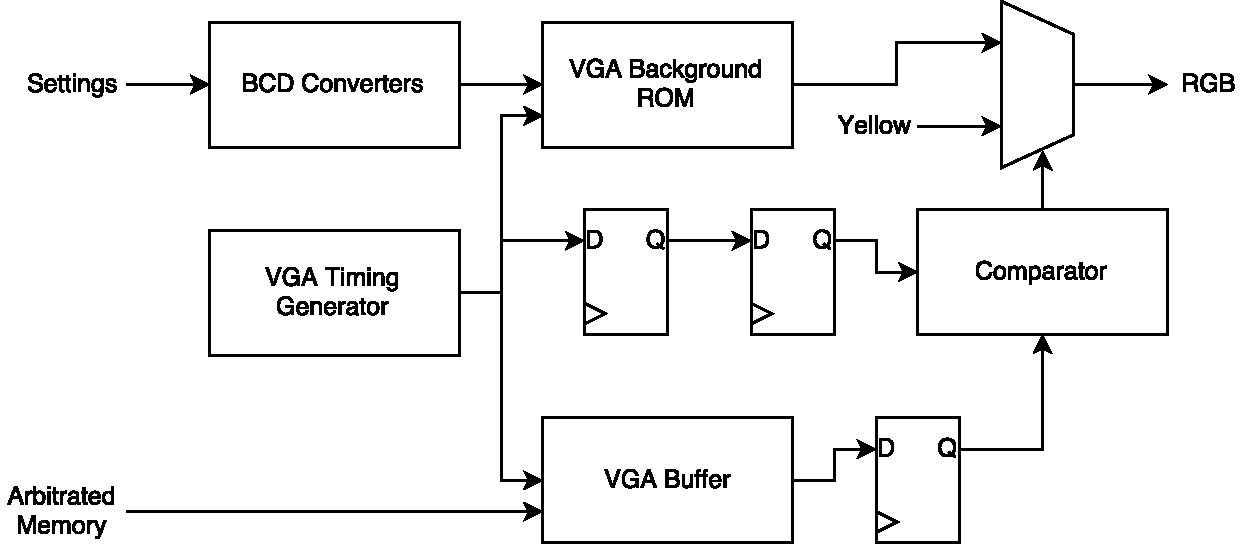
\includegraphics[width=\columnwidth]{diagrams/vga_driver.pdf}
  \caption{Block diagram of the VGA driver module.}
  \label{fig:vga_driver}
\end{figure}

The VGA timing generator entity is used to produce the signals that control the VGA output, such as the VSYNC and HSYNC synchronization signals, the ROW and COLUMN screen position signals, and the BLANK signal for blanking the on-screen data when outside of the visible area.

The VGA buffer entity burst reads the data from the arbitrated memory block when the VSYNC signal goes low. Once completed, it outputs the value of the data for the current COLUMN. In order to allow for vertical interpolation between consecutive data points, it also outputs the subsequent data point. If no such data point exists, it outputs the same data point twice.
These data signals are then passed through a comparator, which determines if the current pixel should be drawn. It does so by checking that the current ROW lies between the two consecutive data points. If it does, it outputs a control signal which sets the output color to yellow for the waveform.

If the current ROW lies outside the consecutive data points, the output color is determined by the VGA background ROM module. This module takes as inputs the VGA timings and the settings and measurements to display on the screen. To allow for conversion between numerical data and ASCII encoding, the measurements and settings are passed through a set of binary-coded decimal (BCD) converters, which convert the numbers into a set of 4-bit decimal digits that can be easily processed. A block diagram of the background ROM module is shown in Figure~\ref{fig:vga_rom}.

\begin{figure}[!htb]
  \centering
  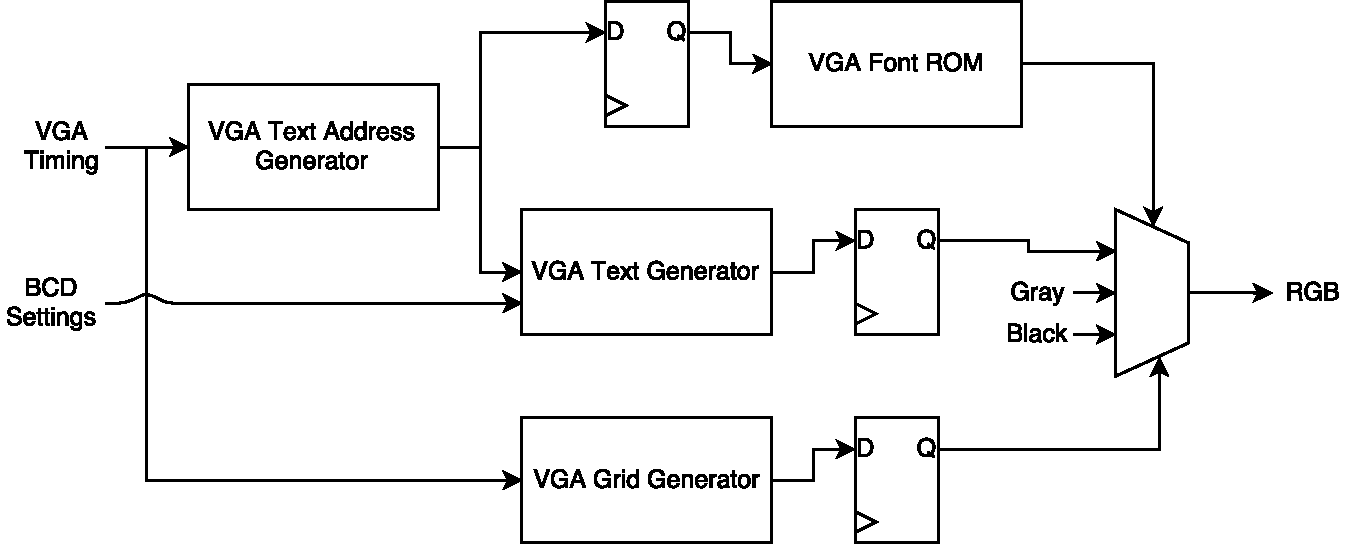
\includegraphics[width=\columnwidth]{diagrams/vga_rom.pdf}
  \caption{Block diagram of the VGA background ROM module.}
  \label{fig:vga_rom}
\end{figure}

To produce the background image, the VGA text address generator entity first converts the ROW and COLUMN values to a new coordinate system better suited to text characters. These coordinates, along with the BCD measurements and settings, are passed to the VGA text generator entity which determines the character to be drawn at the current position. This character then passes to a VGA font ROM which determines if the current pixel should be drawn.
In parallel, the VGA grid generator entity checks the current ROW and COLUMN values and determines if the current pixel corresponds to a point on the waveform grid. If it does, it outputs a control signal to color the current pixel in gray.

For this module, we encountered two main problems. The first was that unequal delay paths between signals led to an improper display of the characters and waveforms on the VGA display. To solve this, we added registers on the faster paths to equalize the delays. The second problem was that the voltage and frequency measurements were being updated too quickly at 72~Hz, resulting in unreadable digits. We solved this problem by limiting the update rate for the data to 4~Hz with a simple counter. We then added a running average for the frequency measurement which takes advantage of the dead time introduced to improve the accuracy of the measurement.

\subsection{Triggering}

Next, we designed the triggering module, which generates a trigger signal in order to achieve a stable waveform display and clear signal characterization. A block diagram of the module can be seen in Figure~\ref{fig:triggering}. The trigger type can be either rising or falling edge, and it controls a comparator which compares the current ADC data, the previous ADC data, and the trigger reference in order to determine if a trigger should occur. For a rising edge trigger type, the previous data should be less than or equal to the reference and the current data should be greater than the reference. For a falling edge trigger type, the previous data should be greater than or equal to the reference and the current data should be less than the reference.

\begin{figure}[!htb]
  \centering
  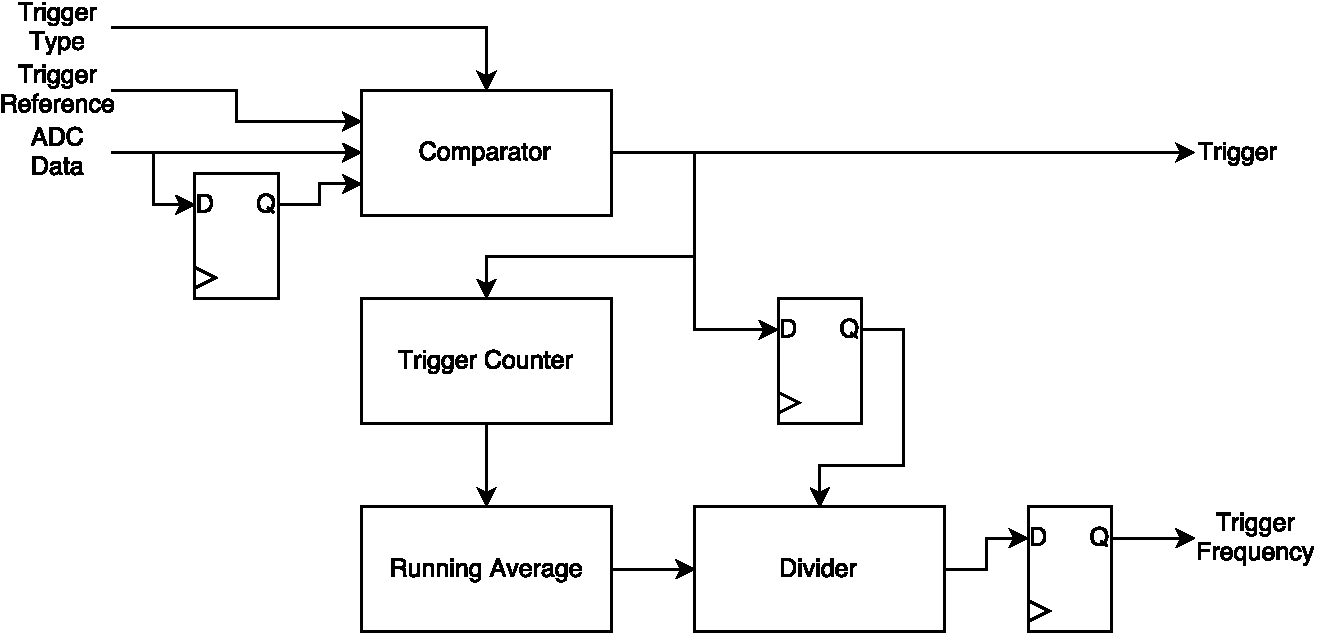
\includegraphics[width=\columnwidth]{diagrams/triggering.pdf}
  \caption{Block diagram of the triggering module.}
  \label{fig:triggering}
\end{figure}

The triggering module also computes and outputs the trigger frequency. It does so through the use of an internal counter which counts the time between trigger signals. The output of this counter is passed through a running average block which reduces the effect of trigger jitter and outputs the trigger period count. When a trigger occurs, the counter is reset and the running average is enabled in order to save the current trigger period count. A delayed trigger signal then enables a multi-cycle divider which divides the clock rate by the average trigger period count in order to obtain the trigger frequency, which is stored in a register and output.

For this module, we encountered two main problems. The first problem was that computing the frequency from the period required division. Using single-cycle division would have reduced our maximum clock rate below our required 50~MHz. To solve this problem, we designed a multi-cycle divider to spread the latency over multiple clock cycles and keep the clock rate high. The second problem was that the waveform would not appear on screen if no triggers were generated. To help the user see the location of the waveform and trigger on it, we decided to add an automatic triggering mechanism. This would generate a trigger signal if one has not occurred for a long period of time. The automatic triggering rate was chosen as half the video frame rate at 36~Hz.

\subsection{Data Acquisition}

We then designed the data acquisition module, which acquires the data sampled by the ADC and writes captured waveforms to an arbitrated memory block when triggered. A block diagram of the module is shown in Figure~\ref{fig:data_acquisition}. The waveform data is stored in an internal RAM block, which is made larger than the maximum captured waveform in order to allow the ADC to sample continuously. In order to prevent loss of ADC sample points, we give full priority to the ADC in terms of access to this RAM block. The ADC sample signal increments the ADC address and writes the current sample point to the RAM by controlling an address multiplexer.

\begin{figure}[!htb]
  \centering
  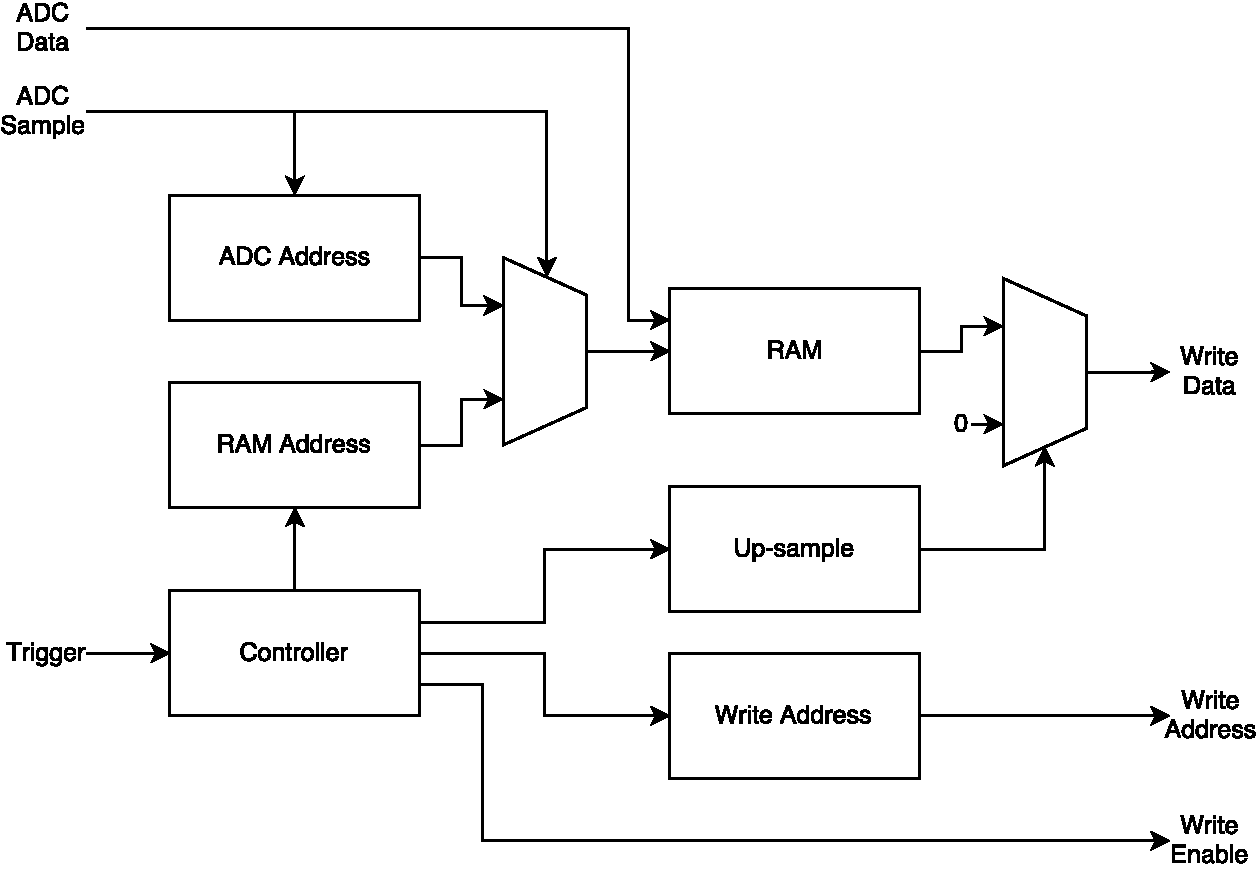
\includegraphics[width=\columnwidth]{diagrams/data_acquisition.pdf}
  \caption{Block diagram of the data acquisition module.}
  \label{fig:data_acquisition}
\end{figure}

The rest of the module consists of the waveform capture blocks. A finite state machine controller waits for a trigger signal to start. Once triggered, it counts the number of points sampled by the ADC until it determines that it has enough data to capture a waveform with the trigger point in the center. It then outputs signals to control the RAM address and write address counters in order to read data from the RAM and output it to an arbitrated memory block.

This controller is also in charge of up-sampling and down-sampling the data. It uses an up-sample counter to output zeros between sample points according to the current horizontal time scale setting. This allows subsequent modules to interpolate the data at these up-sampled points and has the effect of zooming in on the waveform. It also controls the increment of the RAM address counter, which allows it to skip over data to down-sample the waveform.

\subsection{Sin(x)/x Interpolation}

We subsequently designed the interpolation module, which uses a set of low-pass filters to interpolate an up-sampled waveform. A block diagram of the module is shown in Figure~\ref{fig:sinc_interpol}. A finite state machine controller reads the data from an arbitrated memory block and passes it through a filter before saving it in an internal RAM block. It selects the filter to be used based on the current upsample setting. Then, it re-centers the waveform by accounting for the filter delay and burst writes the data to a memory block.

\begin{figure}[!htb]
  \centering
  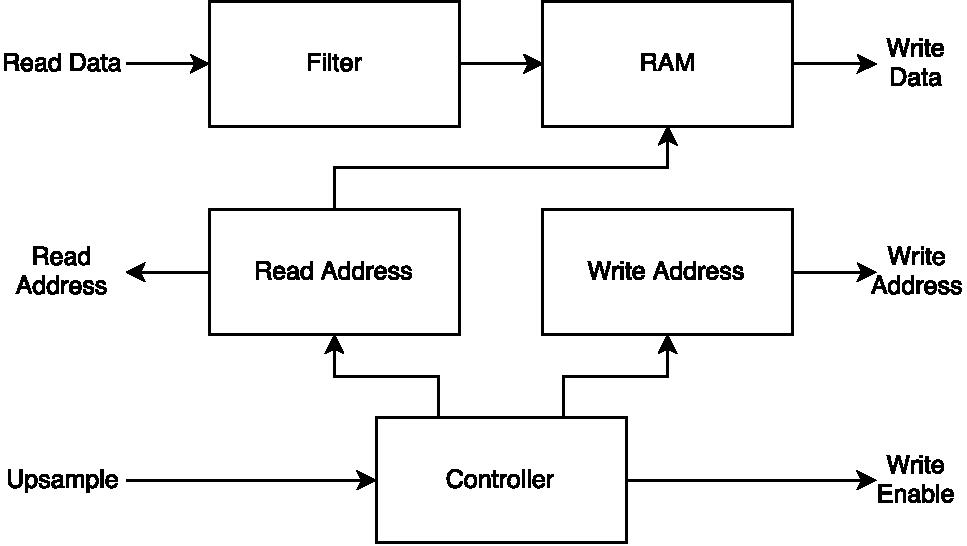
\includegraphics[width=\columnwidth]{diagrams/sinc_interpolation.pdf}
  \caption{Block diagram of the sin(x)/x interpolation module.}
  \label{fig:sinc_interpol}
\end{figure}

One problem we encountered was the size of the filters. We used MATLAB to generate a set of VHDL filters that could interpolate waveforms with up-sampling rates of 2, 4, 8, 16 and 32. However, this design did not fit in our target FPGA, forcing us to remove the 32-point up-sampling rate from our design.

\subsection{Trigger Correction}

Next, we designed the trigger correction module. This module was not originally present in our design and was added later to solve the problem of trigger jitter at high frequencies. The problem is that high frequency signals can only be sampled at a small number of point per period, which results in different trigger points over different periods. To solve this problem, we decided to use the interpolated waveform points to re-center the trigger point. The trigger correction module therefore takes an interpolated waveform and recomputes the center point. A block diagram of the module is shown in Figure~\ref{fig:trig_correction}.

\begin{figure}[!htb]
  \centering
  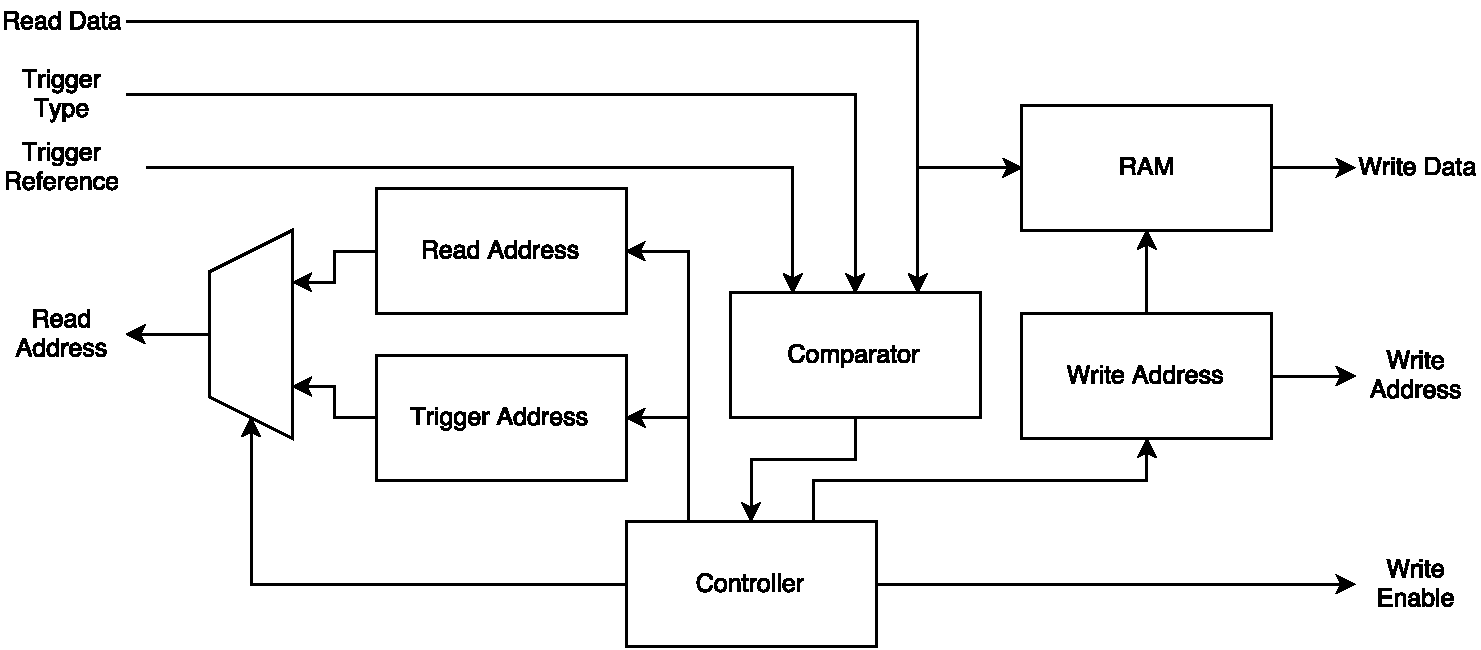
\includegraphics[width=\columnwidth]{diagrams/trigger_correction.pdf}
  \caption{Block diagram of the trigger correction module.}
  \label{fig:trig_correction}
\end{figure}

The module uses a controller and a trigger address to gather the data points located around the center of the waveform. It passes these points, along with the trigger type and reference, through a comparator in order to locate the best point to use as a center point. If it cannot find one, it keeps the previous center point. Once it has determined the new center point, it uses a second address counter to read the data around this point into an internal RAM block. It then writes this data to an external memory block.

\subsection{ADC Interface}

Then, we designed the top-level peripherals that would interact with the development board once synthesized. The main such component was the ADC interface. A block diagram of this interface is shown in Figure~\ref{fig:adc_interface}. The ADC sampler implements the serial protocol required by the ADC. However, this protocol requires a 40~MHz clock in order to obtain our desired sample rate. Therefore, we used a phase-locked loop (PLL) to generate this clock from our 50~MHz clock. This created the problem of transferring data between the two clock domains without synchronization issues. In order to solve this, we used a FIFO queue between the clock domains. This allows the ADC clock to produce data at its own rate. Meanwhile, the system clock can read data whenever the queue is not empty.

\begin{figure}[!htb]
  \centering
  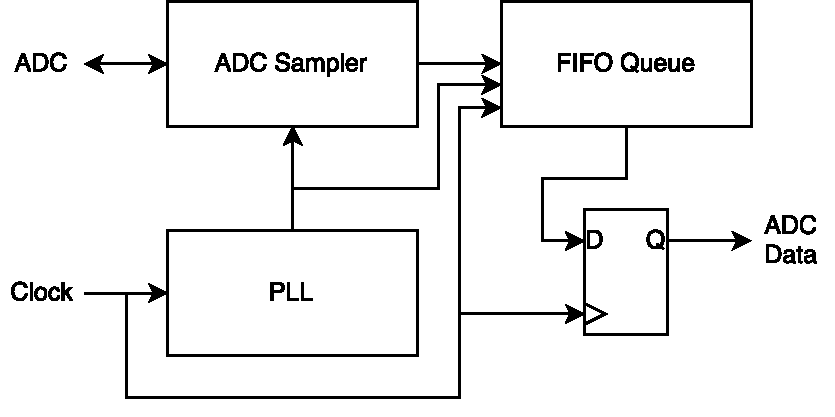
\includegraphics[width=\columnwidth]{diagrams/adc_interface.pdf}
  \caption{Block diagram of the ADC interface.}
  \label{fig:adc_interface}
\end{figure}

\subsection{User Interface}

Finally, we designed an interface to allow the user to control the oscilloscope by using the switches and push-buttons on the DE1-SoC board. This interface is shown in Figure~\ref{fig:ui}. The reset button allows the user to reset the system in case of a glitch. The horizontal timebase is a 3-bit input which varies the horizontal scale from 8~us/div to 1024~us/div in power of 2 increments. The interpolation and trigger correction toggles allow the user to disable these features to demonstrate their effect. The trigger type switch can be either up for rising edge or down for falling edge. Finally, the trigger level push buttons shift the reference level up and down. Each input was passed through a set of two registers to synchronize it to the clock in order to prevent metastability.

\begin{figure}[!htb]
  \centering
  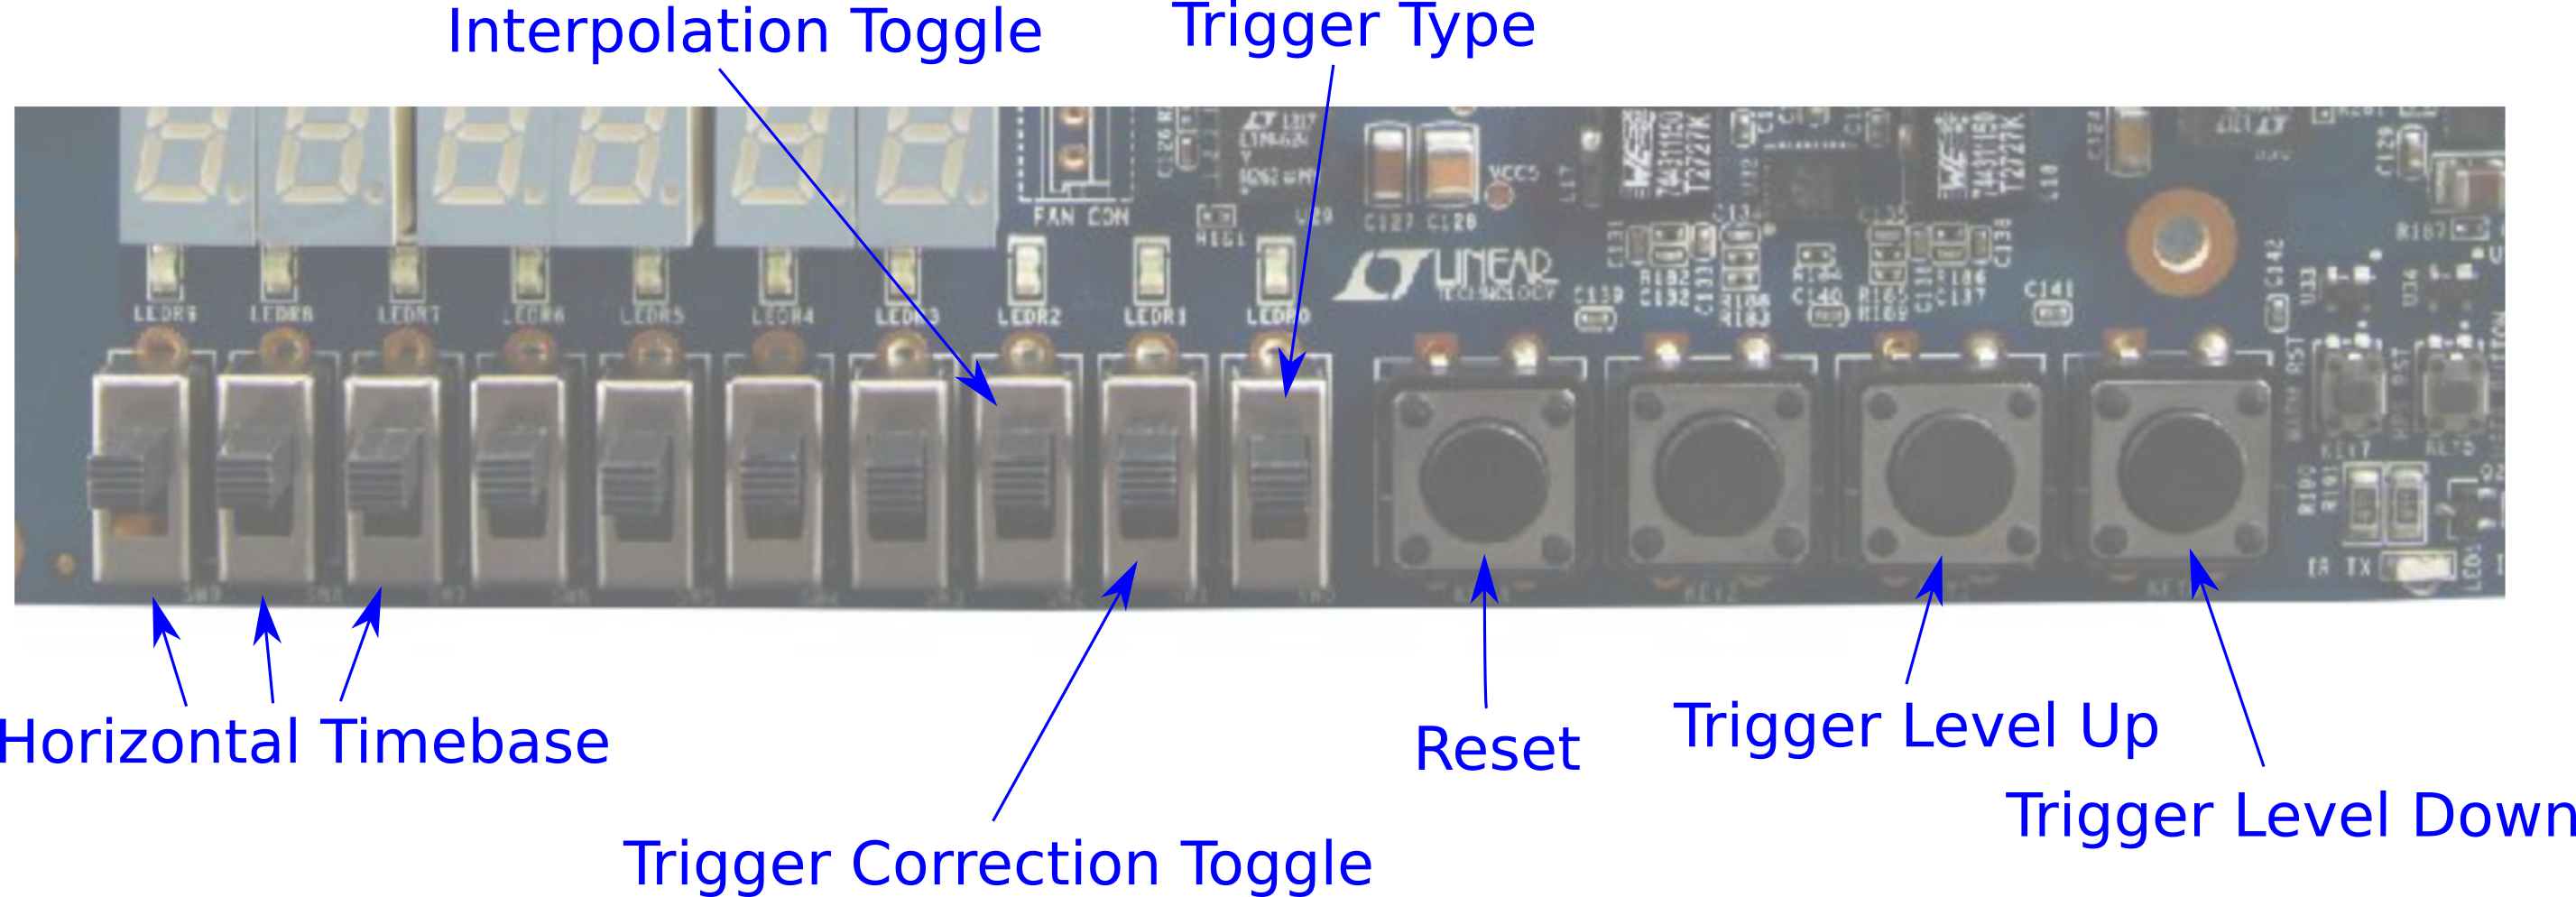
\includegraphics[width=\columnwidth]{diagrams/UI.PNG}
  \caption{User interface for the DSO.}
  \label{fig:ui}
\end{figure}

\section{Results}

In order to ensure proper functioning, every module was tested independently before being combined with other modules to form the system. Most of these tests consisted of checking the outputs of a module against the expected outputs for a set of specified inputs, and these tests were automated to produce a single error count to save us the trouble of checking timing diagrams manually. We therefore describe only the most relevant results here.

First, to test the VGA timings, we created a test-bench which would output a simple array of color bars to the screen. The test-bench was made to log the VGA signals at each clock cycle to a file which we could then view on a VGA simulator. The resulting screen capture is shown in Figure~\ref{fig:vga_timing_test}.

\begin{figure}[!htb]
  \centering
  
\includegraphics[width=\columnwidth]{test-results/vga_timing.png}
  \caption{VGA timing test results.}
  \label{fig:vga_timing_test}
\end{figure}

Then, we tested the entire VGA module by creating a test-bench which connected an arbitrated memory block to the input of the VGA driver. We loaded several test signals into this memory block before the simulation and logged the resulting VGA signals to a text file. We used a simulator to view the resulting display, and the results are shown in Figures~\ref{fig:vga_test_1}~and~\ref{fig:vga_test_2}. Note that the displayed data is for illustration purposes only and does not correspond to real measurements.

\begin{figure}[!htb]
  \centering
  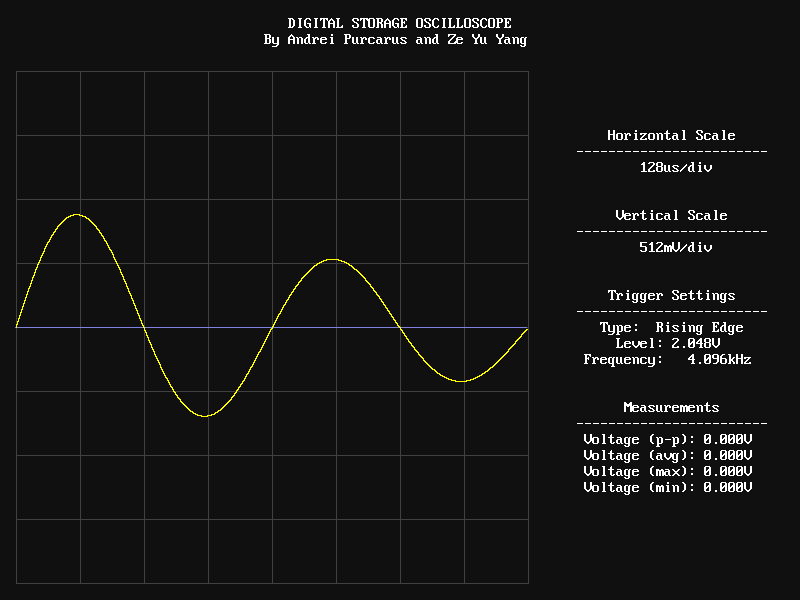
\includegraphics[width=\columnwidth]{test-results/vga_test_signal1.png}
  \caption{VGA driver test results for an exponentially decaying sine wave signal.}
  \label{fig:vga_test_1}
\end{figure}

\begin{figure}[!htb]
  \centering
  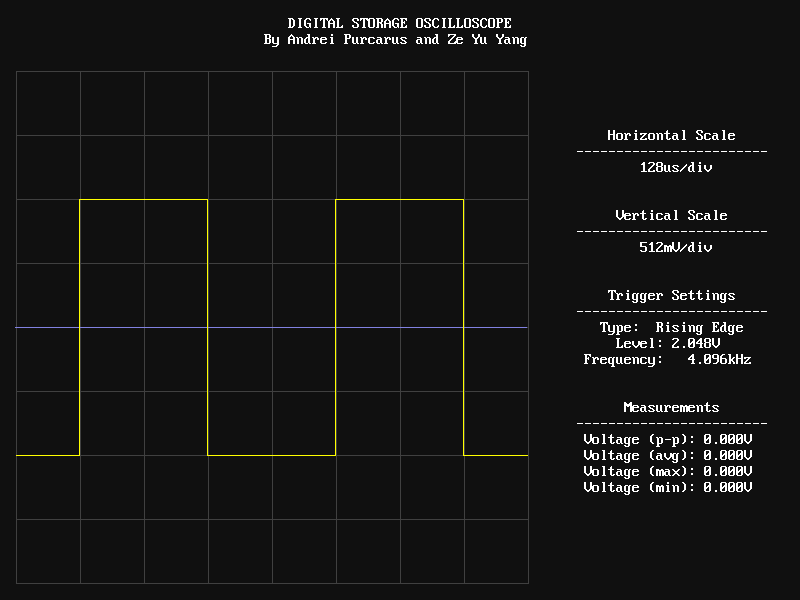
\includegraphics[width=\columnwidth]{test-results/vga_test_signal2.png}
  \caption{VGA driver test results for a square wave signal.}
  \label{fig:vga_test_2}
\end{figure}

Next, we tested the triggering module. We connected the analog waveform generator module we created in a previous assignment to the input of the triggering module and observed the output signals. The resulting timing diagrams are shown in Figures~\ref{fig:trigger_test_1}~and~\ref{fig:trigger_test_2}. From these diagrams, we can see that the module triggers correctly on both rising and falling edges and that the frequency is correctly identified.

\begin{figure*}[!htb]
  \centering
  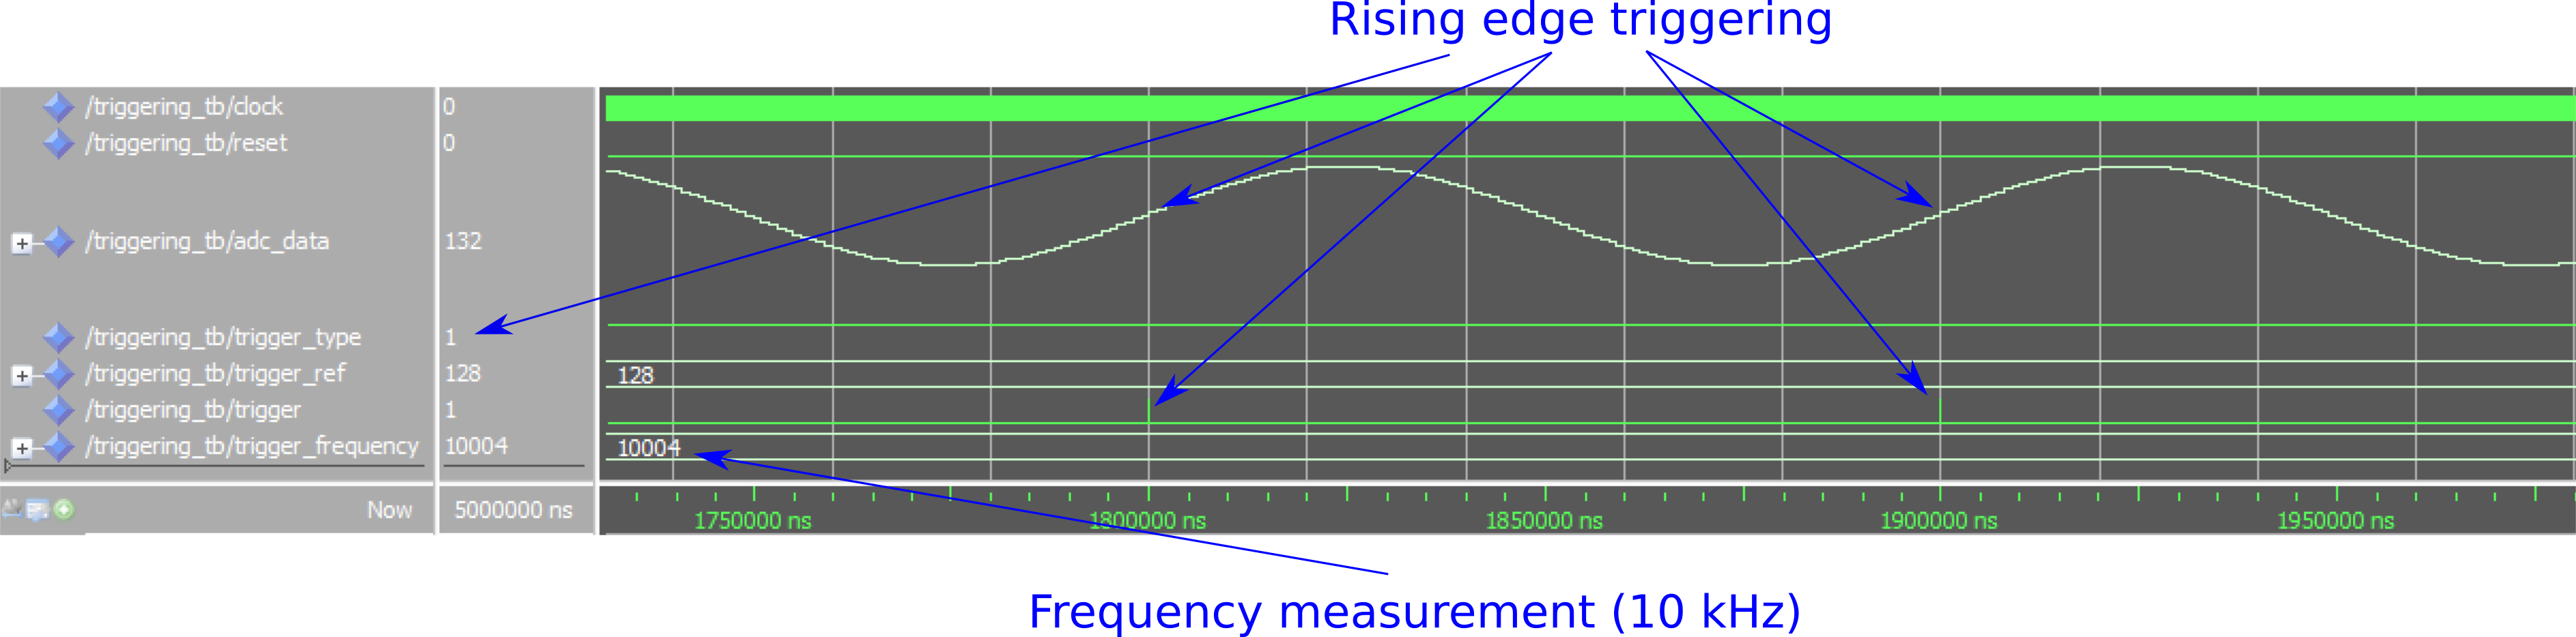
\includegraphics[width=0.8\textwidth]{test-results/trigger_test_rising_10kHz.png}
  \caption{Triggering test results for a rising edge trigger type on a 10~kHz sine wave.}
  \label{fig:trigger_test_1}
\end{figure*}

\begin{figure*}[!htb]
  \centering
  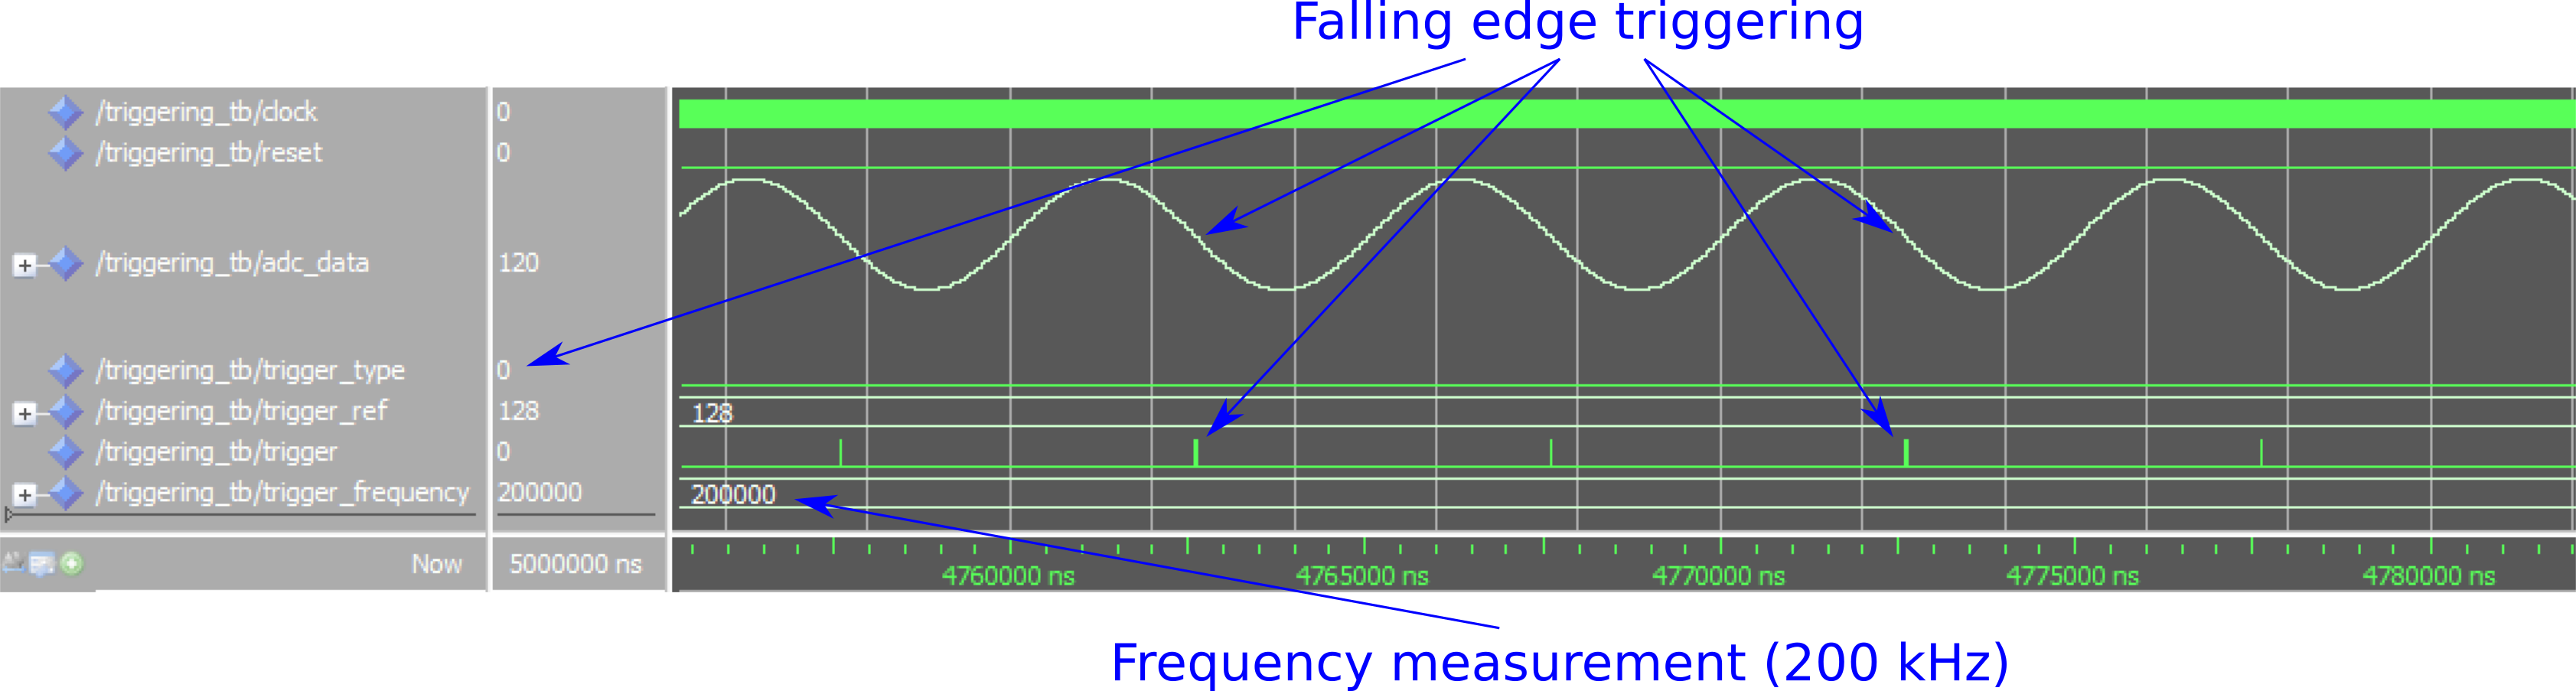
\includegraphics[width=0.8\textwidth]{test-results/trigger_test_falling_200kHz.png}
  \caption{Triggering test results for a falling edge trigger type on a 200~kHz sine wave.}
  \label{fig:trigger_test_2}
\end{figure*}

\begin{figure*}[!htb]
  \centering
  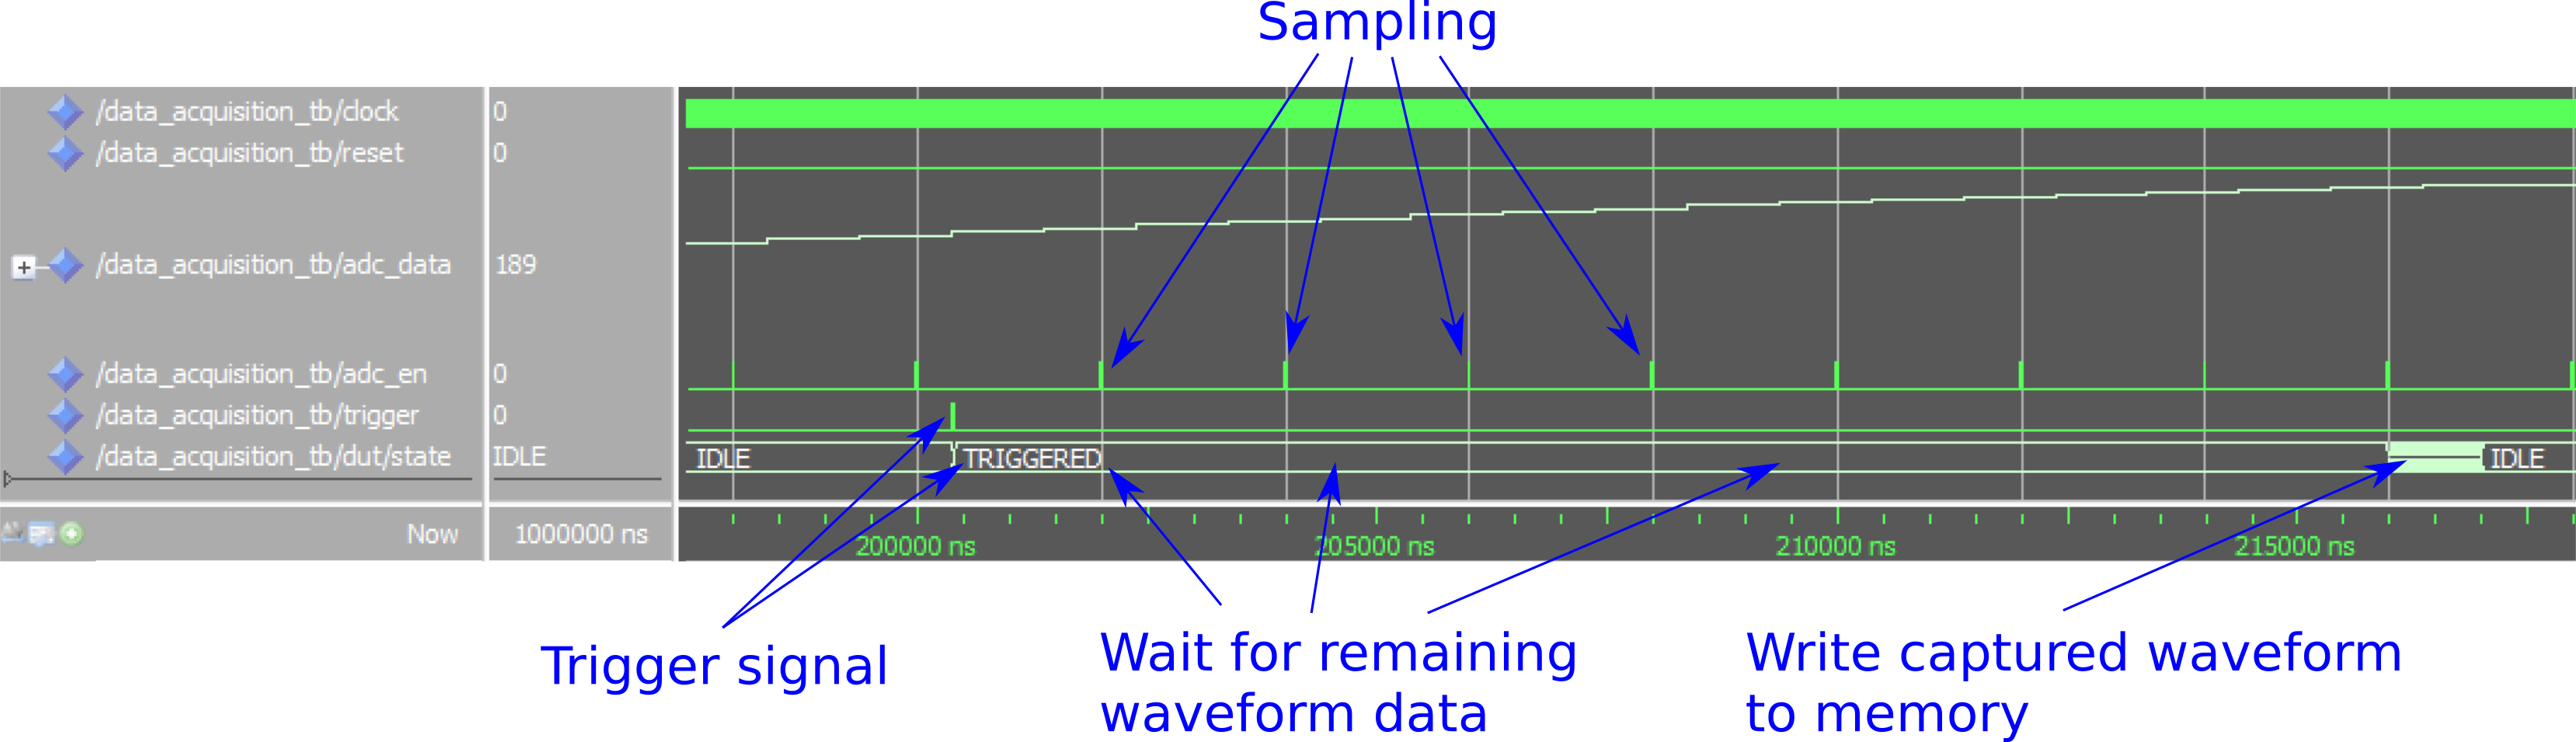
\includegraphics[width=0.8\textwidth]{test-results/data_acquisition_test.png}
  \caption{Data acquisition test results.}
  \label{fig:data_acq_test}
\end{figure*}

We then tested the data acquisition module by connecting the triggering and analog waveform generator modules as inputs and observing the state transitions of the internal controller. The results are shown in Figure~\ref{fig:data_acq_test}. From this figure, we can see that the controller switches into a triggered state when a trigger occurs and waits for sufficient sampled data to be available before burst writing the waveform to memory.

Next, we tested the interpolation module by connecting it to two arbitrated memory blocks. The block connected to the input of the module was preloaded with an up-sampled waveform and the resulting interpolated waveform was read from the output memory block. The results are plotted in Figure~\ref{fig:interpol_test} for an up-sampling rate of 16. This figure shows that the module correctly performs the interpolation and properly re-centers the waveform to account for the filter delay. Note that the time and voltage scales correspond to discrete steps and have no units.

\begin{figure}[!htb]
  \centering
  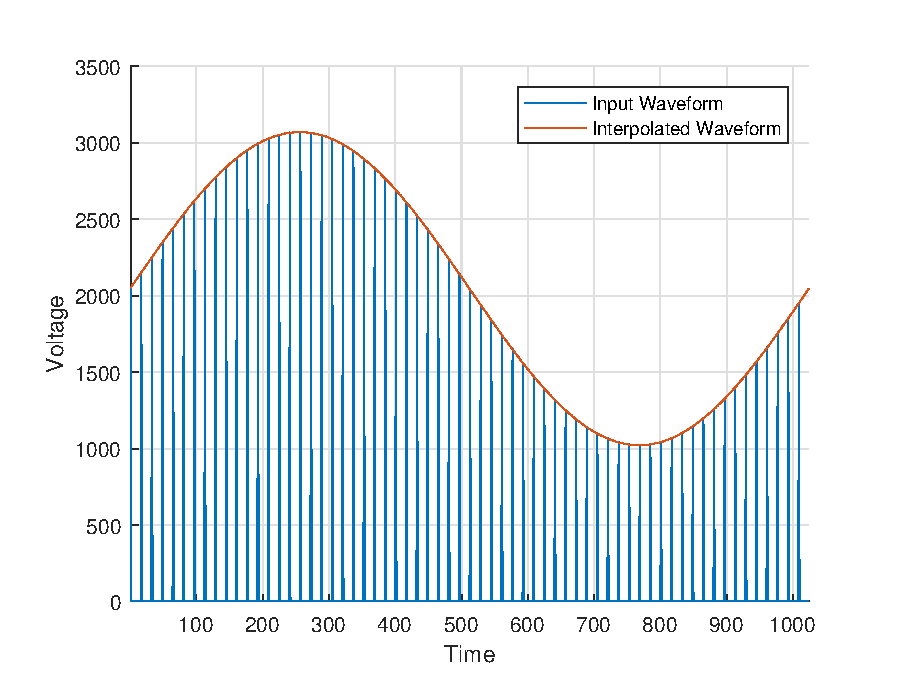
\includegraphics[width=\columnwidth]{test-results/interpolation.eps}
  \caption{Interpolation test results for an up-sampling rate of 16.}
  \label{fig:interpol_test}
\end{figure}

We then tested the trigger correction module by connecting two arbitrated memory blocks to its input and output and preloading shifted waveforms into the input block. We connected the output block to a VGA module and observed the resulting waveforms on a simulator which showed that they were correctly centered. The corresponding screen captures are omitted in this report as they would not contribute to demonstrating this effect.

Next, we combined all the modules together into a top level DSO entity. We then connected the analog waveform generator as an input to the system and observed the resulting VGA outputs for different signal frequencies. The results are shown in Figures~\ref{fig:scope_test_1},~\ref{fig:scope_test_2},~\ref{fig:scope_test_3},~and~\ref{fig:scope_test_4}. Note that the timebase was changed for the different frequencies to show the effects of up-sampling, down-sampling and interpolation. We can see from these figures that the sample points are correctly displayed and the frequency and voltage measurements are correctly computed.

\begin{figure}[!htb]
  \centering
  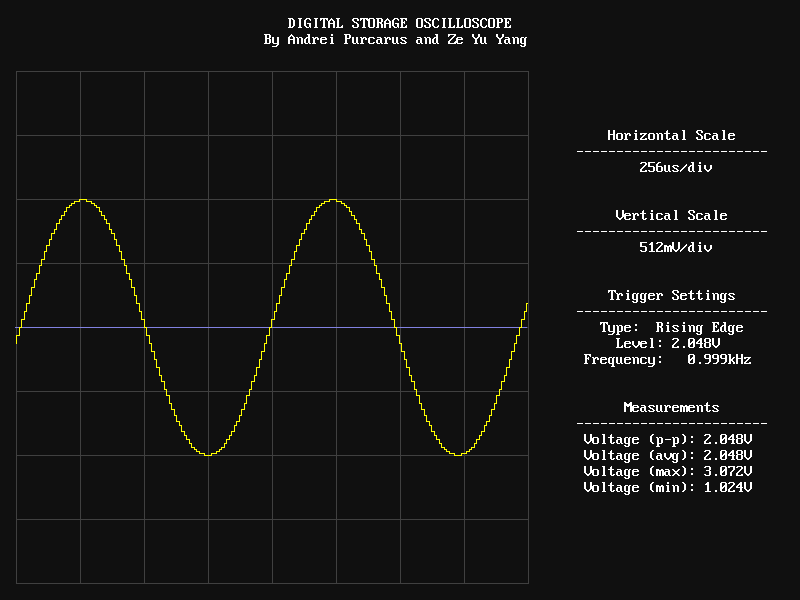
\includegraphics[width=\columnwidth]{test-results/scope_demo_1kHz.png}
  \caption{Oscilloscope test results for a 1~kHz sine wave input on a 256~us/div horizontal scale.}
  \label{fig:scope_test_1}
\end{figure}

\begin{figure}[!htb]
  \centering
  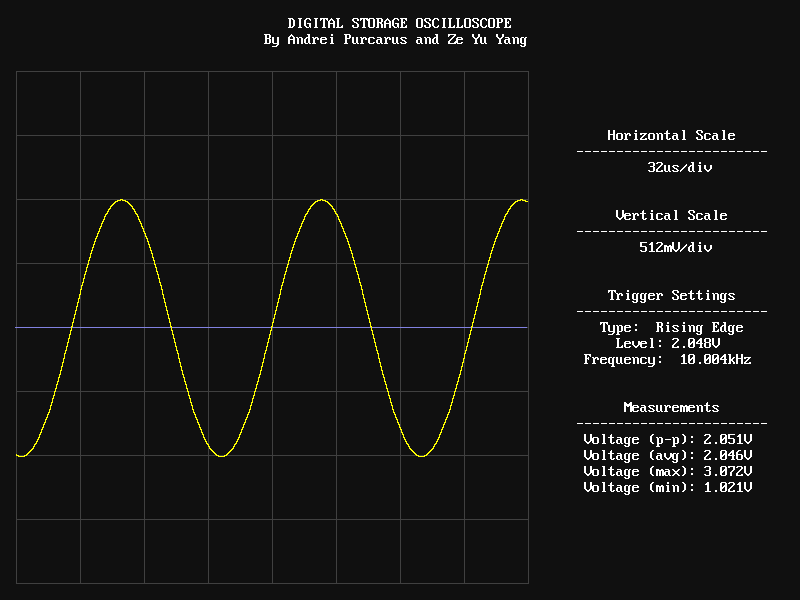
\includegraphics[width=\columnwidth]{test-results/scope_demo_10kHz.png}
  \caption{Oscilloscope test results for a 10~kHz sine wave input on a 32~us/div horizontal scale.}
  \label{fig:scope_test_2}
\end{figure}

\begin{figure}[!htb]
  \centering
  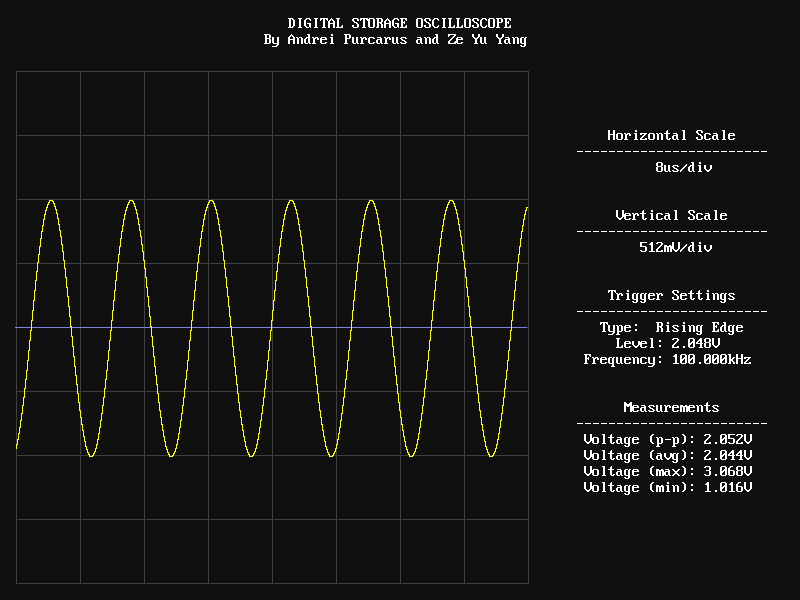
\includegraphics[width=\columnwidth]{test-results/scope_demo_100kHz.png}
  \caption{Oscilloscope test results for a 100~kHz sine wave input on a 8~us/div horizontal scale.}
  \label{fig:scope_test_3}
\end{figure}

\begin{figure}[!htb]
  \centering
  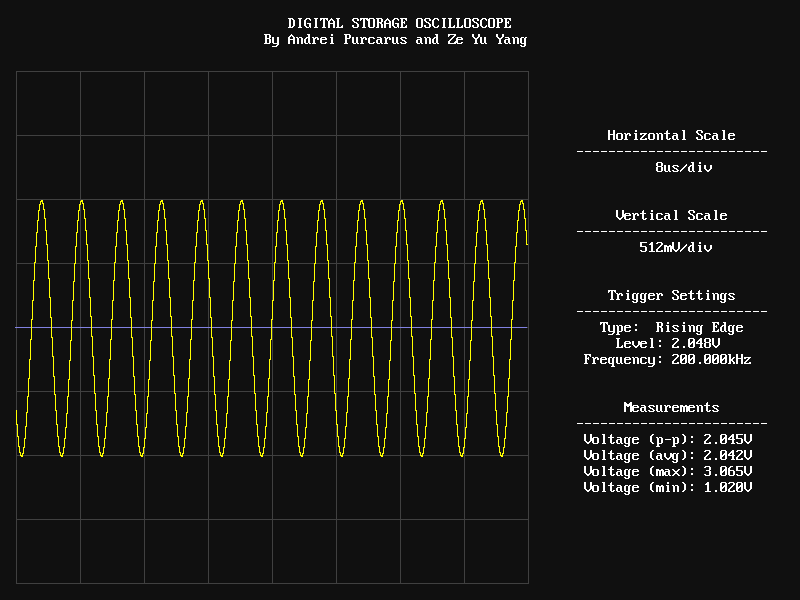
\includegraphics[width=\columnwidth]{test-results/scope_demo_200kHz.png}
  \caption{Oscilloscope test results for a 200~kHz sine wave input on a 8~us/div horizontal scale.}
  \label{fig:scope_test_4}
\end{figure}

We then synthesized the design for the target FPGA. The synthesis results are shown in Table~\ref{tab:synthesis_results}, which shows a maximum clock frequency of 60.26~MHz. This meets our goal of a 50~MHz clock. We can also see that the design uses a large amount of the resources on the FPGA, with a logic utilization of 62~\% and a DSP block utilization of 100~\%. This is a result of the filters used for interpolation requiring a large amount of logic and registers.

\begin{table}[!htb]
  \centering
  \caption{Synthesis results on the Cyclone V 5CSEMA5F31C6 FPGA using a 50~MHz clock.}
  \label{tab:synthesis_results}
  \begin{tabular}[c]{ | l | l | }
    \hline
    \textbf{Family} & Cyclone V \\
    \hline
    \textbf{Device} & 5CSEMA5F31C6 \\
    \hline
    \textbf{Logic Utilization} & 19,901 / 32,070 ( 62~\% ) \\
    \hline
    \textbf{Total Registers} & 23770 \\
    \hline
    \textbf{Total Block Memory Bits} & 246,832 / 4,065,280 ( 6 \% ) \\
    \hline
    \textbf{Total DSP Blocks} & 87 / 87 ( 100 \% ) \\
    \hline
    \textbf{Fmax} & 60.26~MHz \\
    \hline
    \textbf{Setup Slack} & 3.405~ns \\
    \hline
    \textbf{Hold Slack} & 0.016~ns \\
    \hline
  \end{tabular}
\end{table}

We then connected the synthesized oscilloscope board to a function generator and measured the trigger frequency of a waveform over our target range of frequencies. The waveform was chosen to be a 2~V peak-peak sine wave with a 2~V offset in order to provide a reasonable waveform in the center of our vertical range. We compared our results to the frequency counter on a Rigol DS1054Z oscilloscope. The results are shown in Figure~\ref{fig:freq}. We observed a maximum error of 0.26~\%, occurring at a frequency of 161 kHz.

\begin{figure}[!htb]
  \centering
  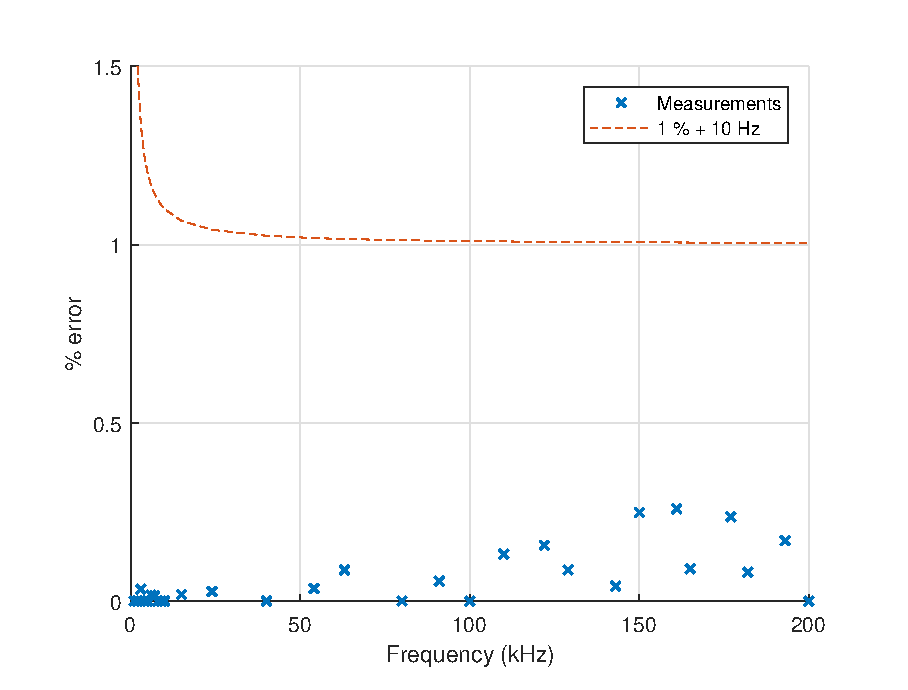
\includegraphics[width=\columnwidth]{test-results/freq.eps}
  \caption{Trigger frequency measurement error when compared to the 6-digit frequency counter on the Rigol DS1054Z oscilloscope.}
  \label{fig:freq}
\end{figure}

Finally, to test the voltage measurements, we decided to test the absolute voltage measurements and the relative voltage measurements of the oscilloscope separately.

To test the absolute measurements, we connected the synthesized oscilloscope board to a DC voltage source and measured the accuracy of the average voltage measurements. We compared our results to the DC voltage readout on a BK Precision 2709B multimeter. The results are shown in Figure~\ref{fig:volt}. We observed a maximum error of 9.6~\%, but this error occurred at a low voltage of 0.104~V and thus the absolute error was not greater than 10~mV.

\begin{figure}[!htb]
  \centering
  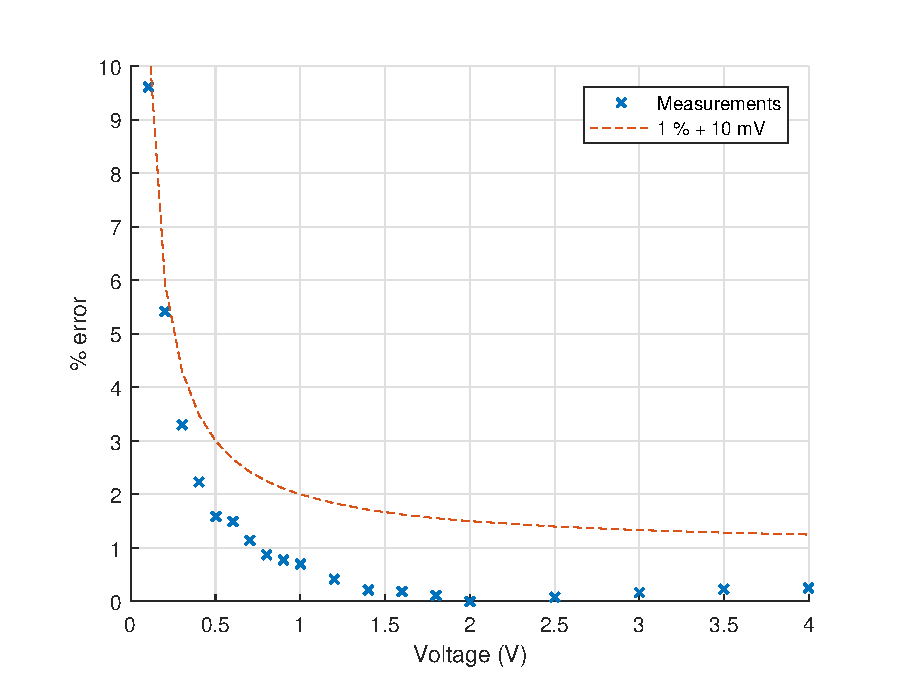
\includegraphics[width=\columnwidth]{test-results/volt.eps}
  \caption{DC voltage measurement error when compared to the BK Precision 2709B multimeter.}
  \label{fig:volt}
\end{figure}

To test the relative measurements, we connected the synthesized oscilloscope to a function generator and measured the accuracy of the peak-peak voltage measurements over the entire frequency range. The input was set to a 2~V peak-peak sine wave with a 2~V offset, and the frequency was swept from 1~kHz to 200~kHz. Since the Rigol DS1054Z oscilloscope specifies a gain error of up to 3~\% for the vertical measurements while the Rigol DG1022Z function generator specifies a maximum error of 1~\%~+~1~mV, the voltage measurements were compared to the DG1022Z readout \cite{ds1054z,dg1022z}. In order to account for variation of the output voltage with frequency, the readouts were scaled by using the DS1054Z oscilloscope measurements. The results are shown in Figure~\ref{fig:voltpp}. This figure shows that the maximum error occurs at 130~kHz, with a value of 1.2~\%. This meets our specification since the combination of maximum relative and absolute errors is greater than the measurement error.

\begin{figure}[!htb]
  \centering
  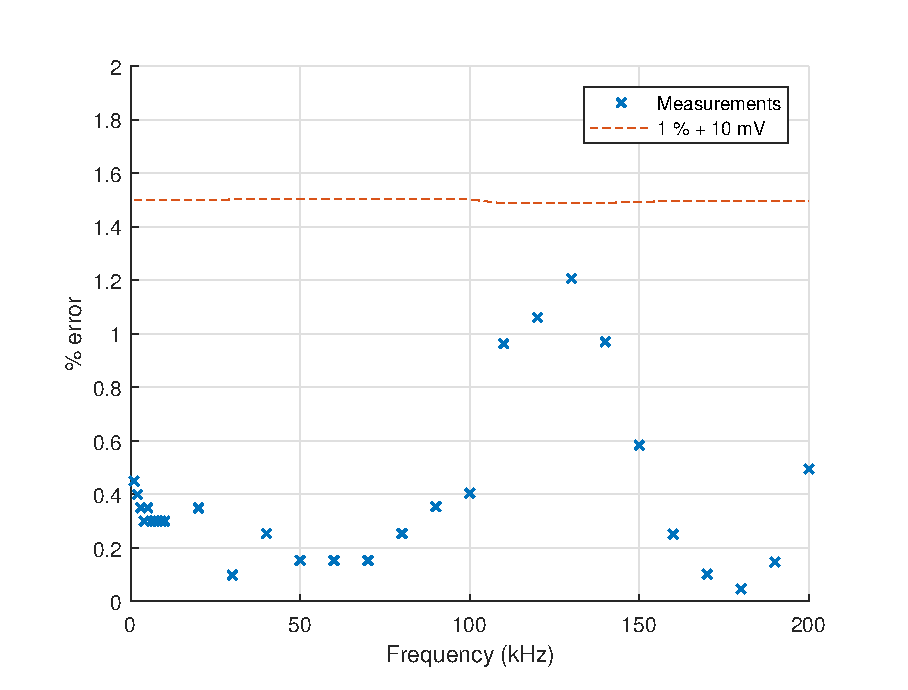
\includegraphics[width=\columnwidth]{test-results/voltpp.eps}
  \caption{Peak-peak voltage measurement error when compared to the scaled readout on a Rigol DG1022Z function generator.}
  \label{fig:voltpp}
\end{figure}

\section{Analysis}

From the results, we can see that our goals have been met. We can correctly interpolate and display waveforms with frequencies up to 200~kHz, as shown in Figures~\ref{fig:scope_test_1},~\ref{fig:scope_test_2},~\ref{fig:scope_test_3},~and~\ref{fig:scope_test_4}.

In addition, the frequency measurements are well within our target accuracy of 1~\%~+~10~Hz, with a maximum relative error of 0.26~\%. We can see from Figure~\ref{fig:freq} that the relative error increases with frequency. This is caused by our limited clock rate. When computing the trigger period, we can only count in steps of 20~ns, as dictated by our clock period. This quantization of measurement reduces the resolution we can obtain at higher frequencies. A possible solution to this problem would be to average the computed frequencies over a period of time, which would increase the resolution of the measurement. However, our current implementation is still an order of magnitude better than what other implementations have achieved with the same hardware resources \cite{jin_digital_2016}.

Also, the absolute voltage measurements produced by our oscilloscope are well within our target accuracy of 1~\%~+~10~mV. We can see from Figure~\ref{fig:volt} that the accuracy is best around the midpoint of the ADC range and deviates at both ends. In particular, the relative error increases to 9.6~\% at a voltage of 0.104~V. However, this still corresponds to less than 10~mV in absolute error.

In addition, the relative voltage measurements produced by our oscilloscope are within our specified accuracy of 1~\%~+~10~mV. We can see from Figure~\ref{fig:voltpp} that the worst case error is 1.2~\%, which is within the tolerance when taking into account the absolute error. We can see that relative voltage measurements are less accurate than absolute ones. This occurs because we are computing the difference between two measurements, which has the effect of doubling the error.

\section{Conclusions}

We implemented the modules required for an FPGA implementation of a digital storage oscilloscope. The current implementation is capable of triggering on a waveform, capturing it and displaying it to a VGA monitor. It is capable of up-sampling or down-sampling a waveform to change the horizontal scale and interpolating between the up-sampled points. It is also capable of producing a stable waveform display over a frequency range of 1~kHz to 200~kHz.

It can measure the trigger frequency, a proxy for the frequency of the waveform, with a maximum error of 0.26~\% over the entire frequency range. It can also measure absolute and relative voltages with a worst case error of 1~\%~+~10~mV over the entire frequency range.

However, there are several improvements which could be implemented. First, the trigger frequency measurement could be improved at high frequencies by providing some additional averaging to increase the resolution. Second, additional trigger modes could be implemented. Traditional DSOs typically provide Normal and Single trigger modes in addition to the Auto mode implemented here. Normal mode consists of only displaying waveforms when an actual trigger occurs and Single mode consists of only capturing a single waveform and displaying it for the user to analyze. These improvements would not use too many resources and would likely fit on the target FPGA.

\bibliographystyle{IEEEtran}
\bibliography{IEEEabrv,references}

\end{document}
